\section{Diseño}
\marginpar{(Pendiente)}

\subsection{Transformador}

La potencia aparente del transformador es la suma de la potencia de entrada y la potencia de salida:

$$ P_{t}=P_{i}+P_{o}=\frac{P_{o}}{\eta}+P_{o}=(1+\frac{1}{\eta})P_{o} $$

La tensión en el bobinado primario está dada por: 

$$ V_{1}=K_{t} f N_{1} \phi_{m} $$

donde $f$ es la frecuencia de conmutación de la señal de entrada y 
$K_t$ es un factor que vale 4.44 si la forma de onda es sinusoidal o 4 si es rectangular.

El flujo se relaciona con el área de la sección transversal de la trayectoria del flujo $A_{c}$ y la densidad de flujo $B$ de la siguiente manera:

$$ \Phi=BA $$

La densidad de corriente es:

$$ J=K_{j} A_{p}^{x} $$

donde $K_{j}$ y $x$ son constantes que dependen del núcleo magnético dadas por la siguiente tabla:

% De que libro es esto? Asi voy pasando las tablas
INSERTAR TABLA!

El factor $A_{p}$ se puede calcular como: 

$$ A_{p}=\left(\frac{P_{t} \cdot 10^{4}}{K_{t} f B_{m} K_{u} K_{j}}\right)^{\frac{1}{1+x}} {cm}^{4} $$

donde $K_u$ es el factor de relleno que varía entre 0.4 y 0.6 y $B_m$ es la densidad de flujo máxima.

La cantidad de alambre de cobre y la cantidad de material del núcleo (por lo general ferrita de hierro) determinan la capacidad de potencia del transformador. 
Existen distintos tipos de núcleo como toroidal, pot, power, E-laminated, EI, C, single-coil, tape-wound, etc. 
En este proyecto se trabajará con los núcleos disponibles provistos por la cátedra: EC70, E42 y E30. 

Especificaciones obtenidas por simulación:
\begin{itemize}
    \item Frecuencia de la forma de onda rectangular: $f=125kHz$
    \item Tensión máxima aplicada a la bobina del primario: $V_{1_{max}}=350V$
    \item Tensión de salida en el secundario: $V_{0}=12.6V$
    \item Corriente de salida en el secundario: $I_{0}=1.6A$
    \item Eficiencia: $n=95\%$
\end{itemize}

INSERTAR IMÁGEN DE SIMULACIÓN V1MAX!

\paragraph{Cálculos}

Potencia de salida:

$$ P_{o}=V_{o}\cdot I_{o}=12.6V\cdot 1.6A=20.16W $$

Potencia aparente: 

$$P_t=P_o+P_i=P_o\cdot\left(1+\frac{1}{n}\right)=20.16W\cdot\left(1+\frac{1}{0.95}\right)=41.38W  $$

% Estoy buscando una decente
INSERTAR IMÁGEN B-H DE KIKE!

En base a las curvas de magnetización se observa como las ferrites no soportan tanto flujo como el hierro y como disminuye la permeabilidad para campos mayores.  
Presenta el ciclo de histéresis y comienza a saturar en B=300mT. 
La saturación implica mayor circulación de corriente que conlleva a que el núcleo deje de responder. 
La saturación se da en campos menores si la temperatura aumenta con el funcionamiento del dispositivo. 
Por lo tanto se elige una inducción magnética máxima de $B_{m}=100mT$ para estar lejos del codo y asegurarnos tener la permeabilidad especificada en las hojas de datos. 

Para el núcleo E70, el área efectiva es: 

$$ A_{e}=279{mm}^{2} $$

Número de vueltas del primario:

$$ N_{1}=\frac{V_{1_{max}}}{K_{t}\cdot f\cdot B_{m}\cdot A_{a}}=\frac{350V}{4\cdot 125kHz\cdot 100mT\cdot 0.000279}=25.09\simeq 25 $$

Número de vueltas del secundario: 

$$ N_{2}=N_{1}\cdot\frac{V_{2}}{V_{1}} $$

Como no se requiere ni desea elevar o reducir la tensión del secundario, se elige una relación de vueltas 1:1. 
Por lo tanto, el número de vueltas del bobinado secundario es igual al del primario. 

$$ N_{2}=25 $$

$$ A_{p}=\left(\frac{41.38\cdot 10^{4}}{4\cdot 125kHz\cdot 100mT\cdot 0.4\cdot 366}\right)^{\frac{1}{1-0.14}} {cm}^4 $$

$$ J=366\cdot X^{-0.14} A/{cm}^2 $$

$$ J=584 A/{cm}^2 $$

\paragraph{Saturación magnética}

Cualquier componente de continua puede causar la saturación magnética del núcleo, 
elevando la corriente magnetizante. 
Para minimizar los efectos de la saturación, se puede utilizar un núcleo más grande o incluir un entrehierro.
El entrehierro permite que exista en el núcleo, además de una zona con alta permeabilidad propia del material magnético, 
otra zona de baja permeabilidad propia del espacio de aire. 
De esta forma en condiciones normales el flujo circula por el material magnético y en caso de saturación circula por el entrehierro 

\subsection{Inductor}

Se utiliza para almacenar energía y permitir su transferencia. 
Por el inductor circula una corriente continua. Si la misma es muy elevada puede saturar el núcleo magnético. 

Requisitos de diseño: 

\begin{itemize}
    \item Inductancia: $L=400\mu H$
    \item Corriente continua: $I_{dc}=1A$
\end{itemize}

Procedimiento para el diseño de un inductor con entrehierro:

\paragraph{Calculo la energía que debe almacenar el inductor}
$$ E=0.5\cdot L\cdot I_{dc}^2=200\mu HA^2 $$
\paragraph{Elección el tamaño del núcleo}
En base a la disponibilidad, se elige un E30 con material N27. 
Sus parámetros son:
\begin{itemize}
    \item Longitud efectiva: $l_e=67mm$
    \item Área efectiva: $A_e=60{mm}^2$
    \item $A_l=1800nH$ y $u_e=1600$ ($gap=0mm$)
    \item $A_l=630nH$ y $u_e=562$ ($gap=0.1mm$)
    \item $A_l=400nH$ y $u_e=353$ ($gap=0.18mm$)
    \item $A_l=200nH$ y $u_e=179$ ($gap=0.34mm$)
\end{itemize}

\paragraph{Verificar energía almacenada}

Se debe corroborar que la energía que puede almacenar el inductor sin entrehierro sea suficiente

Con $B_m=100mT$:
$$ E_{singap}=\frac{0.5\cdot B_m^2\cdot {volumen}}{u_0\cdot u_e}=\frac{0.5\cdot B_m^2\cdot A_e\cdot l_e}{u_0\cdot u_e}=10\mu HA^2 $$

Con $B_m=200mT$:
$$ E_{singap}=\frac{0.5\cdot B_m^2\cdot {volumen}}{u_0\cdot u_e}=\frac{0.5\cdot B_m^2\cdot A_e\cdot l_e}{u_0\cdot u_e}=40\mu HA^2 $$

En ambos casos es menor a la energía que debe almacenar el inductor por lo que se evidencia la necesidad de incluir un entrehierro. 

\paragraph{Dimensionar el entrehierro}

El entrehierro $l_0$ debe almacenar la energía $E$ con $B_{max}=100mT$.
En caso de ser necesario puede llevarse a $B_{max}=200mT$ sin problema. 

Con $B_m=100mT$:
$$ l_0=\frac{2\cdot E\cdot u_0}{A_e\cdot B_m^2}=0.84mm $$

Con $B_m=200mT$:
$$ l_0=\frac{2\cdot E\cdot u_0}{A_e\cdot B_m^2}=0.2mm $$

Gap necesario con un núcleo tipo E:

Con $B_m=100mT$:
$$ g=\frac{l_0}{2}=0.42mm $$

Con $B_m=200mT$:
$$ g=\frac{l_0}{2}=0.1mm $$

\paragraph{Dimensionar el número de vueltas}

Elección de N para conseguir la inductancia L requerida.

Con $B_m=100mT$:
$$ N=\sqrt{\frac{L\cdot l_0}{A_e\cdot u_0}}=67\ vueltas$$

Con $B_m=200mT$:
$$ N=\sqrt{\frac{L\cdot l_0}{A_e\cdot u_0}}=34\ vueltas $$

\paragraph{Construcción}

Bobinar el inductor y medir L. Si no verifica el valor deseado corregir
considerando $L = A_LN^2$ (el valor de $A_L$ que corresponde a $l_0$ se obtiene con
el número de vueltas del primer intento).

Mediante la constante de tiempo en un circuito RL con una forma de onda cuadrada a la entrada se estima la inductancia en $L=450\mu H$. 

\paragraph{Validación}

Verificar que el valor de L se mantiene con la corriente de DC de trabajo.
Esto generalmente se realiza sobre el propio convertidor midiendo la
tensión aplicada sobre el inductor y la pendiente de la corriente.

\subsection{Driver}

1) Tensión de control de puerta: Vdrv

Es la amplitud de la forma de onda PWM:  

Vdrv=8V

2) Frecuencia de control de puerta: fdrv

Es la frecuencia de conmutación: 

fdrv=125kHz;

3) Carga total del terminal Gate: Qc

Una de las principales pérdidas de potencia en los transistores MOSFET son las pérdidas por control de puerta o Gate. 
El encendido y apagado del MOSFET implica la carga y descarga del capacitor interno, 
el cual recibirá o entregará carga cuando la tensión en el mismo se modifique. 
Se requiere de una cierta carga para cambiar la tensión del terminal Gate entre 0 y Vdrv. 
Su valor se obtiene mediante el gráfico de la hoja de datos del IRF840 con los siguientes datos:
Rango: 0-63nC
Vgs=6V
Vds=100V
De forma estimada: 
Qg=26nC

INSERTAR IMÁGEN DE HOJA DE DATOS IRF840: FIGURA 6 Vgs vs Qg

Con este parámetro pueden determinarse la corriente promedio de polarización requerida para controlar el terminal Gate 
y las pérdidas de potencia de carga de puerta

Ig=Qg*fdrv=3.25mA

Pgate=Vdrv*Qg*fdrv=26mW

4) Delta VC1 y Delta VC2: INSERTAR SÍMBOLOS COMO ANTES

La suma de los ripples en ambos capacitores de acoplamiento aparece en el terminal Gate. 
Se elige el siguiente criterio:
DeltaVc=0,1*Vdrv
deltavc1=deltavc2=deltavc/2;

5) Tensión del diodo de rueda libre del secundario: Vdc2

Se utiliza el mismo diodo que en el convertidor forward, modelo UF4007. 
La tensión directa máxima se obtiene de la hoja de datos: 
Vdc2=1.7V;

6) Ciclo de trabajo máximo 

Definido por el conversor forward.

Dmáx=0.5

7) Resistencia entre Gate y Source: Rgs

Su valor se despeja en base a la constante de tiempo deseada en el transitorio de la tensión en el capacitor de acoplamiento.

Tao=50us

INSERTAR CÁLCULO DE RGS

$Rgs=10k\Omega$

8) Inductancia magnetizante: Lm

Medida con el instrumento. 

Lm=186uH;

9) Cdrv: Capacitor de bypass

Provee de la corriente necesaria al encenderse. 

FALTA CÁLCULO

INSERTAR FÓRMULA DE LA ECUACIÓN 18 JUNTO A LA DESCRIPCIÓN DE SUS parámetros

10) Capacitor de acoplamiento Cc1

$$ C_{C_1}(D)=\frac{Q_g}{\Delta V_{C_1}}+\frac{(V_{drv}-V_{{dc}_2})\times D}{\Delta V_{C_1}\times R_{gs}\times f_{drv}}+\frac{V_{drv}\times (D^2-D^3)}{\Delta V_{C1}\times 4\times L_m\times f_{drv}^2} $$

La capacidad mínima que asegura permanecer por debajo del ripple de tensión máximo en todas las condiciones de operación 
se puede encontrar determinando el máximo de la expresión anterior:

Cc1=328.3nF

11) Capacitor de acoplamiento Cc2

Cc2=(Qg/deltavc2)+(((Vdrv-Vdc2)*Dmax)/(deltavc2*Rgs*fdrv))

Cc2=71.3nF

12) Resistencia serie del primario de amortiguamiento

$Rcmin=2*sqrt(Lm/Cc1)=47.6\Omega$

Se elige:

Rc=X

\subsubsection{Diseño del conversor}

El primer paso de diseño fue la elección de una topología de conversión DC-DC.
Esta etapa introduce aislación a partir de un transformador de alta frecuencia,
disminuyendo el coste, tamaño y peso respecto a uno de baja frecuencia en base al núcleo magnético necesario.
Como se requiere una única tensión de salida se evita utilizar múltiples devanados.
El conversor debe alcanzar una potencia máxima de 300W y debe ser lo más sencillo posible para evitar un costo elevado. 

La topología flyback es de baja complejidad al estar integrada por muy pocos componentes. 
Como desventajas, el tamaño del núcleo del transformador se incrementa con la potencia requerida y en bornes del
interruptor presenta una tensión igual al doble de la tensión máxima de entrada.
En aplicaciones típicas se alcanzar valores de hasta 150W.

La topología forward con un solo switch disminuye el tamaño del núcleo del transformador ya que la energía no necesita almacenarse en el entrehierro.
Como desventajas, al igual que el flyback presenta alta tensión en bornes del interruptor y se eleva el costo debido al agregado de la bobina de filtrado.
La topología forward con dos switches reduce la tensión en bornes del interruptor a la mitad respecto a la de un solo switch (y con ello la disipación de potencia por switch), 
pero el circuito de excitación de uno de los transistores queda flotante respecto a masa. 
La topología con un solo switch admite una potencia de salida entre 150-250W y con 2 switches se eleva a 500W \cite{mohan}\cite{hart}. 
En base a los criterios definidos inicialmente se eligió el conversor forward con dos switches como topología de conversión DC-DC. 

El principal problema que presentó la utilización de este conversor fue que las señales que controlan a los switches son poco convencionales.

\subsubsection{Simulación del rectificador de entrada AC-DC}
Una vez definido el circuito de conversión DC-DC, se procedió a analizar los requisitos de la tensión de entrada. 
Los circuitos rectificadores AC-DC permiten convertir una tensión alterna en una tensión continua.

\paragraph{Rectificador de media onda u onda completa}

Si bien el rectificador de media onda es más simple ya que cuenta con un menor número de diodos, existen muchas ventajas del rectificador de onda completa frente al de media onda. 
La primera de ellas es que la corriente media del generador de alterna (alimentación) es nula, lo cual beneficia a los transformadores. 
La segunda se basa en el hecho de que para una misma carga,
la tensión de rizado pico a pico para el rectificador de onda completa es
aproximadamente la mitad que para el rectificador de media onda. 
Esto se debe a que en el circuito de onda completa,
el tiempo durante el que se descarga el capacitor es menor que en el circuito de media onda
debido a la onda sinusoidal rectificada de la segunda mitad de cada período. 

Por todos estos motivos se decidió implementar un rectificador de onda completa.

\paragraph{Rectificador de onda completa en puente o con toma media}

\paragraph{En puente}

Presenta la caída de tensión de 2 diodos entre el generador y la carga. 
La tensión máxima en un diodo polarizado en inversa es el valor pico del generador.

\paragraph{Transformador de toma media}

Sólo presenta la caída de tensión de un diodo entre el generador y la carga. 
Para una misma potencia entregada por el generador,
los diodos consumen potencia y disminuyen la corriente y potencia que absorbe la carga. 
La tensión máxima en un diodo polarizado en inversa es el doble del valor pico del generador.
El transformador proporciona aislamiento eléctrico entre el generador y la carga. 

Como la reducción de tensión a la salida no es significativa en esta aplicación
y el puente de diodos se puede implementar con un pequeño integrado,
con el objetivo de disminuir el tamaño del circuito se decidió evitar el transformador
y utilizar un rectificador de onda completa tipo puente.

\paragraph{Filtrado}
% ¿No usamos bobina?
El filtro pasa bajos compuesto por una red LC permite disminuir el rizado,
es decir, la componente de alterna de la señal rectificada. 
Como resultado se logra una tensión de salida aproximadamente continua.
El capacitor mantiene la tensión de salida en un nivel constante y
la bobina suaviza la corriente del rectificador y reduce la corriente de pico en los diodos. 

Para disminuir el número de componentes se decidió utilizar únicamente
un capacitor en paralelo con la capacidad suficiente para obtener una tensión continua.

\paragraph{Rectificación controlada}

Los tiristores son interruptores electrónicos controlados que son activados por una señal externa. 
Poseen 3 terminales: ánodo, cátodo y puerta. Presentan altos valores nominales de corriente y tensión.
Soportan altas corrientes y altas tensiones de bloqueo. 
Un ejemplo de tiristores con los rectificadores controlados de silicio(SCR).
Para que conduzcan se los debe polarizar en directa y deben recibir una corriente de puerta. 
Al entrar en conducción no es necesaria la señal de puerta para mantener la corriente de ánodo. 
El SCR continuará conduciendo siempre que la corriente de ánodo sea positiva y esté por arriba de un valor mínimo. 
Mediante conmutadores controlados como los SCR se controla la tensión de salida en un rango limitado de variación, ajustando el ángulo de disparo de cada SCR. 
El ángulo de disparo es el intervalo angular entre la polarización directa del SCR y la aplicación de la señal de puerta. 
Si el ángulo de disparo es 0, el comportamiento es igual al de un rectificador no controlado con diodos. 

Se decidió utilizar rectificación no controlada ya que no se necesita una tensión específica a la salida
y el costo de complejizar el diseño con el agregado de SCRs y un circuito dedicado de disparo no aporta ningún beneficio significativo.

\subsubsection{Circuito de control}
Esta etapa fue la mas extensa en diseñar debido a su complejidad.
Inicialmente solo debía realimentar la tensión de salida y generar la señal PWM en base a esta,
pero en base a los cambios descritos en la sección \ref{subsection:estudio_bibliografia}
se separó su diseño en tres etapas:

\begin{enumerate}
    \item Compensador y generador PWM
    \item Selector de modo de funcionamiento
    \item Controlador para los switches
\end{enumerate}

La primer etapa se implementó en base a las topologías descritas en \cite{mohan}. Se puede observar,
en la figura \ref{fig:esquema_compensador}, un modelo simplificado del circuito.

\begin{figure}
    \centering
    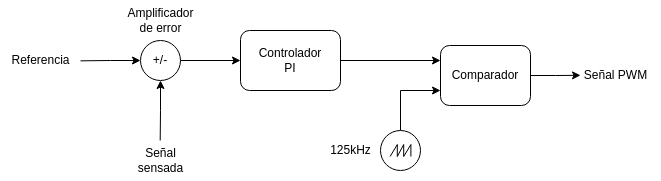
\includegraphics[width=\textwidth]{images/compensador.png}
    \caption{Esquema del compensador y el generador de señal PWM}
    \label{fig:esquema_compensador}
\end{figure}

Los parámetros del bloque proporcional-integrador (PI) fueron definidos a partir de valores típicos obtenidos de \cite{mohan}
y posteriormente ajustados para que el circuito funcione en las condiciones de la aplicación.
La frecuencia de switching es definida por la frecuencia de la señal de diente de sierra y también se tomó un valor típico.

\begin{figure}
    \centering
    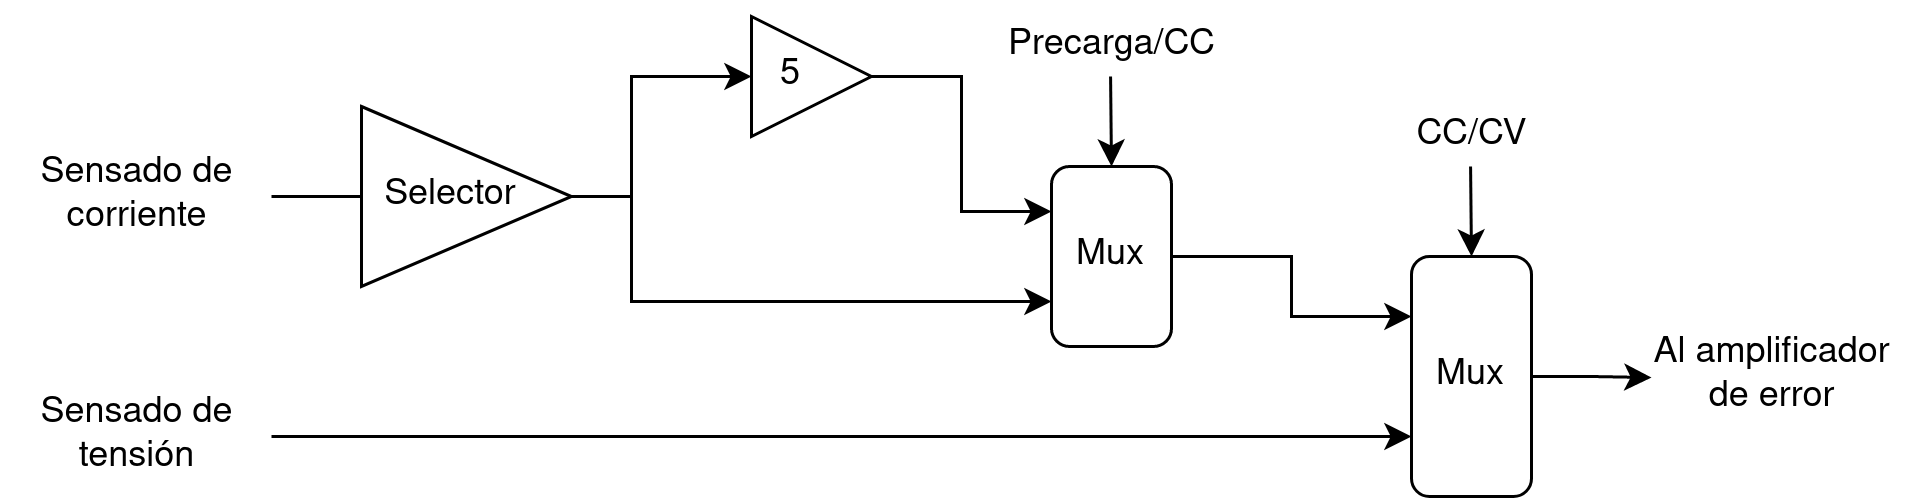
\includegraphics[width=\textwidth]{images/selector.png}
    \caption{Esquema del selector de modo}
    \label{fig:esquema_selector}
\end{figure}

Una vez diseñado el compensador, se procedió a diseñar el circuito de cambio de modo (Precarga, tensión constante y corriente constante).
En la figura \ref{fig:esquema_selector} se puede observar el esquema de este circuito.

Las señales de tensión y corriente están normalizadas con respecto a sus valores nominales.
Un amplificador de ganancia variable actúa como selector de corriente de salida,
modificando la amplitud de la señal de control de dicha variable.
La selección entre el modo de precarga y el modo de corriente constante se hace comparando el nivel de tensión de la batería
con una señal de referencia, siendo el segundo modo activado una vez que la tensión supera los 30V.
El bloque de ganancia 10 tiene como objetivo amplificar la señal de control, ya que la corriente de salida para el modo
de precarga es 10 veces mas chica que la de corriente constante.

La normalización de las señales nombrada anteriormente permite que la selección de la señal del último multiplexor
se haga en base a cual es la mayor de las dos. Esto, visto desde una perspectiva general, permite establecer un límite
tanto de tensión como de corriente de salida, lo cual es importante porque representa la base del método de carga.

Finalmente, para la selección de un controlador para los MOSFETs se tuvieron en cuenta algunos parámetros como
la tensión máxima de entrada, frecuencia de switching y sincronización de las señales,
pero no se logró hallar un controlador adecuado para esta aplicación.
El principal motivo fue que los controladores convencionales generan señales alternadas mediante el método de bootstrapping \cite{hart},
lo cual no sirve para la topología elegida. Esto, combinado con el elevado nivel de tensión en la entrada,
llevó a la búsqueda de otros métodos de control; por eso, se optó por un controlador con transformador aislante para el MOSFET cuyo source no esta a tierra \cite{gatedrivers}. El diagrama de este driver puede observarse en la figura \ref{fig:driver}.

\begin{figure}
    \centering
    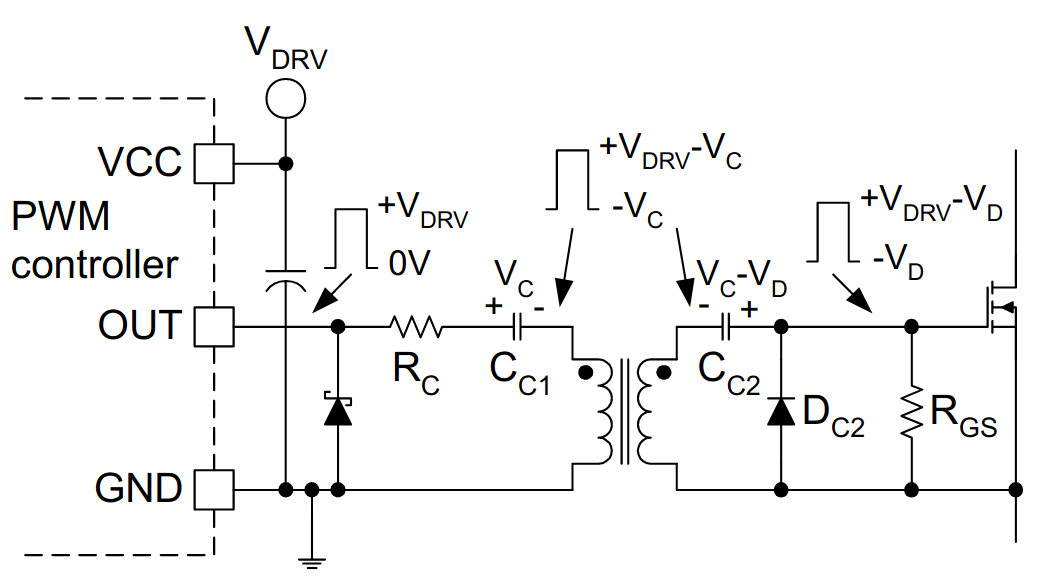
\includegraphics[width=\textwidth]{images/esquema_driver.png}
    \caption{Esquema del controlador del MOSFET high-side}
    \label{fig:driver}
\end{figure}

\subsection{Convertidor Forward}

Las especificaciones del prototipo son las siguientes:

Tensión de entrada: Vs=36V
Tensión de salida: Vo=12.6V
Ciclo de trabajo mínimo: Dmín=0
Ciclo de trabajo máximo: Dmáx=0.5
Frecuencia de conmutación: f=125kHz
Corriente media en la carga: Iprom=1A

Se desea obtener:

Variación en la corriente del inductor: deltaiL=25\%
Ripple de tensión de la salida: deltav=0.2\%

En consecuencia:

DeltaiL=Iprom*(deltai[\%]/100)=1A*(25/100)=0.25A
DeltaVo=Voprom*(deltav[\%]/100)=12.6V*(0.2/100)=0.025V

En principio se dimensiona el filtro de salida compuesto por el inductor y el capacitor. 
En base a la variación de la corriente en el inductor se calcula la inductancia.
Para el ciclo de trabajo mínimo se obtiene la inductancia máxima:

L=[Vo*(1-D)]/(f*DeltaiL)=[12.6V*(1-0)]/(125kHz*0.25A)=400uH
$$ $$

En base a la ecuación de la tensión de rizado pico a pico en la salida se calcula la capacidad.
Para el ciclo de trabajo mínimo se obtiene la capacidad máxima:

C=[(1-D)*Vo]/(8*L*DeltaVo*f^2)=[(1-0)*12.6V]/[8*400uH*0.025V*(125kHz)^2]=10uF
$$ $$

Los dispositivos semiconductores fueron elegidos en base a su disponibilidad en el ATEI,
comprobando que puedan ser utilizados en el prototipo con los parámetros otorgados en su hoja de datos.  

Diodos rectificadores ultra rápidos para alta frecuencia modelo UF4007. 
Presenta tiempo de recuperación inversa ultra rápido, una baja caída de tensión directa, alta capacidad de sobretensión, bajas pérdidas de conmutación y alta eficiencia.
Sus características principales son: 
Máxima corriente rectificada directa promedio: If=1A
Voltaje inverso pico repetitivo máximo: Vrrm=1000V
Tiempo máximo de recuperación inversa: trr=75ns
Tensión directa instantánea máxima: Vf=1.7V

Para los transistores se eligieron MOSFETs para switching de alta velocidad modelo IRF840. 
Sus características principales son: 
Pmáx=125W
Vdsmáx=500V
En base a la tensión rectificada por la etapa de AC-DC, debe soportar 350V. 
Vgsmáx=20V
Idmáx=8A
Idrepetitivamáx=32A